\documentclass[conference]{IEEEtran}
\IEEEoverridecommandlockouts
% The preceding line is only needed to identify funding in the first footnote. If that is unneeded, please comment it out.
\usepackage{cite}
\usepackage{amsmath,amssymb,amsfonts}
\usepackage{algorithmic}
\usepackage{graphicx}
\usepackage{textcomp}
\usepackage{xcolor}
\usepackage[spanish]{babel}
\usepackage[utf8]{inputenc}

\def\BibTeX{{\rm B\kern-.05em{\sc i\kern-.025em b}\kern-.08em
    T\kern-.1667em\lower.7ex\hbox{E}\kern-.125emX}}
\begin{document}

\title{Desarrollo de un software de estimulación visual para estudios electrofisiológicos en primate
despierto\\
}

\author{\IEEEauthorblockN{1\textsuperscript{st} Luis Felipe Llamas Luaces}
\IEEEauthorblockA{\textit{Facultad de Informática} \\
\textit{Universidade da Coruña}\\
A Coruña, España \\
l.f.llamas@udc.es}
\and
\IEEEauthorblockN{2\textsuperscript{nd} Juan Casto Rivadulla Fernández}
\IEEEauthorblockA{\textit{Grupo de Neurociencia y Control Motor} \\
\textit{Universidade da Coruña}\\
A Coruña, España \\
casto.rivadulla@udc.es}
}

\maketitle

\begin{abstract}

El desarrollo de las ciencias de la computación ha impulsado mucho la investigación en neurociencia, especialmente en lo que se refiere a estudios electrofisiológicos y de psicofísica. Esto es debido a la capacidad de presentar estímulos y capturar datos de respuesta con cada vez mayor precisión temporal. Desde los años 70 han aparecido múltiples herramientas que permiten a los investigadores desarrollar experimentos que involucran tanto sistemas de presentación de estímulos como de captura de datos neuronales. En este artículo se presenta Stimpack, una nueva herramienta basada en la librería Psychtoolbox para el entorno Matlab. Stimpack permita a los investigadores el desarrollo de estudios electrofisiológicos en primates de una manera simple y con un entorno gráfico amigable, permitiendo el control de los experimentos a tiempo real. Además Stimpack, proporciona métodos para poder expandir la herramienta mediante la adición de nuevas tareas de forma sencilla. 

\end{abstract}
\begin{IEEEkeywords}
Psicofísica, Neurofisiología, Neurociencia, Vision, Software
\end{IEEEkeywords}

\section{Introducción}
\subsection{Contexto}


%- Si todas la memorias de trabajo son iguales y en que lugar del cerebro se codifican

%- Hipotesos -> dos memorias de trabajo, una sensorial y una conceptual

%- La memoria sensorial debe estar codificada en las áreas visuales(en este caso) en general en las áreas sensoriales. Ej, sin flecha

%- La memoria conceptual esta codificada en el área prefrontal, por ejemplo tarea con flecha


%- Necesidad del proyecto: Simplificar el proceso , tener una herramienta propia elimina dependencias del desarrollador de opticka. 


%- Cortex: Alta comunicación con los miembros del equipo de desarrollo

%- Plexon OnlinePlexonmap? En el ordenador con windows

%- En la introducción explicar la necesidad de fijación, desplazamiento de los campos receptores


%Mapeo

%- Se va a bloquear con tms en el prefrontal, la idea es que a nivel de comportamiento se va a inhibir una de las memorias. Si quitamos prefrontal el resto van a poder codificar la sensorial pero no la conceptual.


%- Se ha probado con los investigadores y la van a usar


%- Explicar que esta disponible en GitHub

%- Trabajo futuro, a través del feedback de otros usuarios, que la herramienta termine siendo algo más general y no solo especifica para este proyecto



El grupo de Neurociencia y Control Motor de la universidad de la Coruña (NeuroCom) lleva a cabo una línea de investigación sobre estudios electrofisiológicos en primates despiertos\cite{neurocom1}\cite{neurocom2}. Actualmente se está desarrollando un proyecto de investigación que intenta descubrir como se organiza y distrubuye la memoria de trabajo en la corteza cerebral. La memoria de trabajo u operativa es aquella encargada del almacenamiento temporal de información que, al contrario que la memoria a largo plazo, toma parte en procesos más complejos en el procesamiento de información. Esta memoria tiene poca capacidad, está en constante cambio y es la encargada de mantener en mente los datos mientras realizamos una tarea.

La hipótesis del proyecto en curso es que hay dos tipos diferentes de memoria de trabajo, la sensorial, que únicamente integra datos de los sentidos y la conceptual, que asocia un significado adicional a estos datos. Lo que se busca demostrar es que la zona sensorial del cerebro, en este caso en la corteza visual ya que los estímulos son visuales, debe tener un papel importante en la codificación de la memoria sensorial mientras que la memoria conceptual se codifica en la corteza prefrontal.
Para comprobar esta hipótesis se diseñó un experimento que permitiera capturar los datos de las zonas implicadas en este tipo de memoria durante la realización de distintas tareas para después inhibir la actividad en la corteza prefrontal y comprobar si la memoria conceptual se ve afectada.

El experimento involucra un primate (un macaco, Macaca mulatta) al que se le mostraran distintos estímulos a través de la vista teniendo que reaccionar usando sus ojos, cuyas reacciones se medirán mediante un sistema de seguimiento ocular. El animal tendrá fija la cabeza mediante una silla específica para esta tarea y se le colocará en frente de un monitor donde se le presentarán los distintos estímulos. Al lado del monitor se encuentra la cámara de seguimiento ocular y un iluminador de infrarrojos para la misma. Adicionalmente cuenta con un sistema de recompensas automático que administra una recompensa en forma de zumo de frutas al animal cuando realiza la tarea correctamente. El animal cuenta con electrodos implantados en las zonas del cerebro a estudiar, a través de los cuales se capturarán los datos de actividad neuronal. Para la inhibición de la corteza prefrontal se usa un sistema de estimulación magnética transcraneal (TMS). Puede verse un esquema del sistema en la figura \ref{figMono}.

Es necesario que la cabeza del animal y la vista del mismo permanezcan fijas en la misma posición para poder estimular con precisión los campos receptores de la corteza visual, para ello, además del sistema de fijación de la cabeza, se debe entrenar al animal para que mantenga la mirada en todo momento en un punto de fijación que aparecerá durante todo el experimento en el centro de la pantalla.


En el grupo actualmente se emplea la herramienta Opticka\cite{opticka} para realizar las diferentes tareas, sin embargo se desea desarrollar una nueva herramienta más especifica para este proyecto, y que además pueda expandirse para futuros desarrollos. La mayor ventaja del desarrollo de una herramienta propia es evitar la dependencia con los desarrolladores de Opticka para implementar cambios en la herramienta y al hacerla más especifica en vez de abarcar muchas cosas permite simplificar la interacción del usuario con la misma.

\begin{figure}[tp]
\centerline{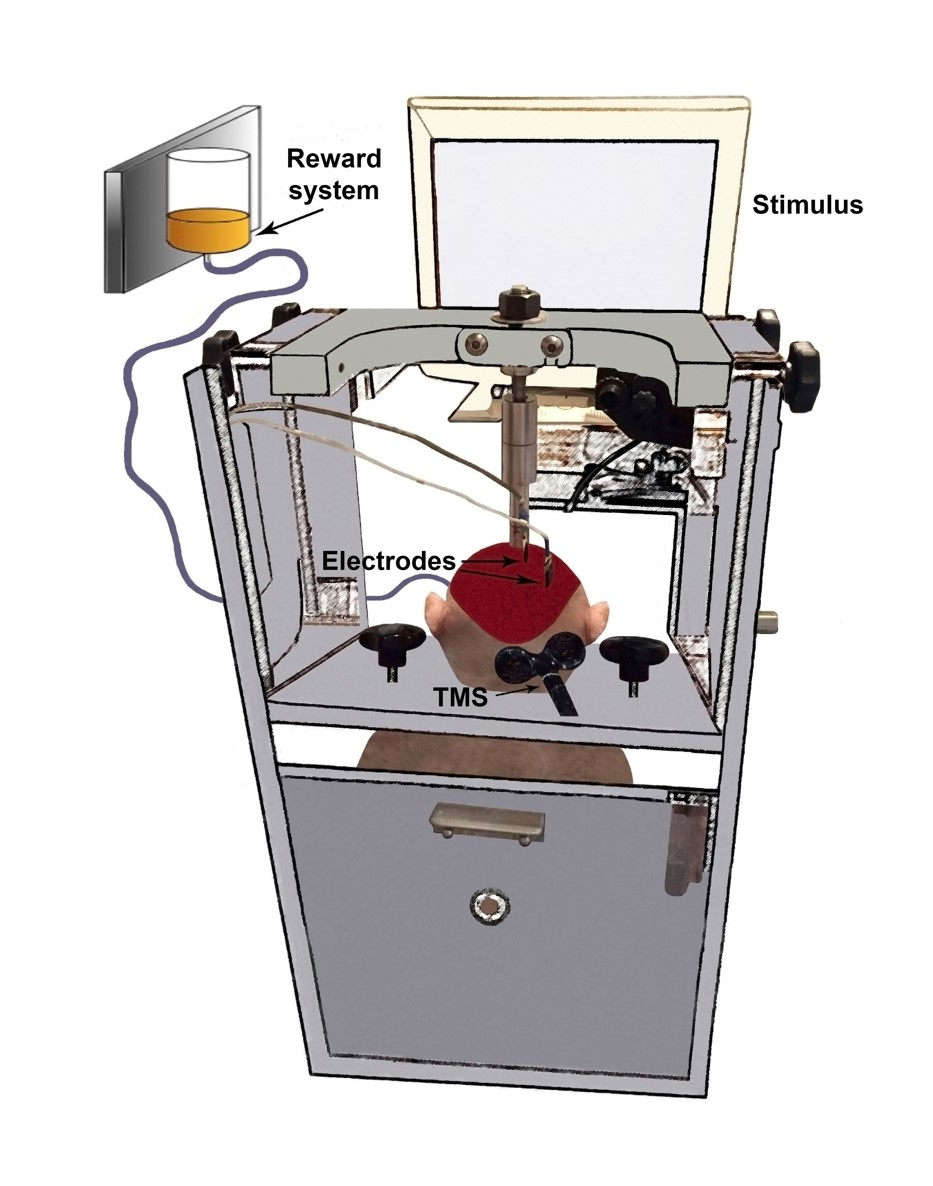
\includegraphics[width=\linewidth]{figures/mono}}
\caption{Configuración del experimento.}
\label{figMono}
\end{figure}
\subsection{Objetivos del proyecto}

Para el desarrollo del estudio mencionado en la sección anterior, es necesario que los investigadores cuenten con una herramienta acorde a sus necesidades. Actualmente los estudios se llevan a cabo empleando la herramienta Opticka, potente, pero al mismo tiempo complicada de usar, con una interfaz de usuario bastante densa y difícil de modificar, haciendo que el trabajo que deben realizar los investigadores no sea tan ágil como les gustaría. Por ello decidieron que la mejor opción era el desarrollo de una herramienta que se adaptara a sus necesidades de forma específica y les fuera fácil de modificar y extender según fueran surgiendo nuevas necesidades.

Hubo un primer intento por parte del grupo de desarrollar una herramienta, Orion, pero no se llegó a utilizar nunca. Esto es debido a que a pesar de estar muy simplificado con respecto a la herramienta anterior, el ajuste de los experimentos se realizaba modificando variables en el propio código de la herramienta, siendo un problema para los investigadores que no están familiarizados con la programación en Matlab. Esta herramienta permitía cierto grado de control a tiempo real del experimento usando comandos de teclado. Otra de las desventajas de Orion era que dependía de parte del código de Opticka para funcionar.


Dado el fracaso de Orion se propone el desarrollo de una nueva herramienta que pueda ser usada por los investigadores sin necesidad de conocimientos de programación y que simplifique el proceso del desarrollo de experimentos.


Por tanto, el objetivo de este proyecto es producir una herramienta que:

\begin{itemize}
	
	\item Permita la presentación de estímulos visuales parametrizables.
	\item Se integre con el sistema de registro de movimientos oculares.
	\item Se integre con el sistema de registro electrofisiológico.
	\item Se integre con el sistema de recompensa.
	\item Cuente con un entorno gráfico amigable.
	\item Pueda ser expandida en un futuro con facilidad.
\end{itemize}

Durante la fase de definición de requisitos del proyecto se hizo especial mención a la necesidad de generar un entorno amigable, por lo que se buscó limitar al mínimo las interacciones con la herramienta a través del teclado y la consola de comandos en favor del uso de un entorno gráfico.

La primera versión de esta herramienta además debe soportar la ejecución de las siguientes tareas experimentales:

\begin{itemize}
	\item Fijación, para el entrenamiento del sujeto.
	\item Mapeo, para localizar los campos receptores en la corteza visual.
	\item Memoria de trabajo, para el estudio de el efecto de la estimulación magnética transcraneal sobre la memoria de trabajo.
\end{itemize}

Estas tareas se explicaran con mayor detenimiento en el apartado de desarrollo.

\section{Trabajo relacionado}

Existen múltiples herramientas para realizar experimentos de estimulación visual, a menudo desarrolladas por los propios grupos de investigación a medida de sus necesidades. A continuación se comentan algunas de las herramientas más relevantes relacionadas con la herramienta desarrollada en este trabajo.

\subsection{Cortex}

Cortex (COmputerized Real Time EXperiments)\cite{cortex} fue una de las primeras herramientas desarrolladas para la ejecución de experimentos neurofisiológicos y de comportamiento en PC.
La herramienta estaba pensada en torno al concepto de ensayo, donde se ejecutaban las diferentes tareas de forma individual mientras los diferentes sistemas de adquisición de datos capturaban la información necesaria, seguidos de un tiempo entre ensayos durante el que se almacenaban los datos y se preparaba el siguiente ensayo. 
La configuración de los ensayos se llevaba a cabo mediante tres archivos de texto que eran importados por Cortex: un archivo de \textit{items} donde se describen los estímulos visuales que se usarán en el experimento, un archivo de condiciones que controla lo que ocurre en cada ensayo y un script de temporización que controlaba los tiempos del experimento. Además de todas las características ofrecidas por la herramienta, Cortex contaba con la ventaja de tener un equipo de desarollo que mantenía un alto grado de comunicación con los usuarios, permitiendo integrar mejoras a la aplicación y dar soporte a los usuarios.


\subsection{Monkeylogic}

\begin{figure}[tp]
\centerline{\includegraphics[width=\linewidth]{figures/monkeylogic.jpg}}
\caption{Interfaz de ususario de Monkeylogic.}
\label{figMonkeyLogic}
\end{figure}

Monkeylogic\cite{monkeylogic} es una herramienta escrita en  Matlab que permite el desarrollo de estudios psicofísicos con una alta precisión temporal, integrando la presentación de estímulos visuales con múltiples tipos de entrada de información del sujeto, como pueden ser sistemas de seguimiento ocular, joysticks o entradas de teclado.
Sus características más destacadas son:
\begin{itemize}
	\item Alta precisión temporal en la presentación de estímulos. 
	\item Interfaz gráfica basada en Matlab para diseño de tareas con flexibilidad.
	\item Compatibilidad con múltiples modelos de hardware de adquisición de datos.
	\item Interfaz de ejecución de experimentos con información a tiempo real del comportamiento y rendimiento del sujeto.
	\item Estructura de programación de experimentos derivada de la de CORTEX\cite{cortex} mediante un archivo de condiciones y un script de temporización.
	\item Las tareas pueden ser modificadas durante la ejecución de las mismas.
\end{itemize}
Esta herramienta se utiliza de forma extensa, siendo una de las herramientas de este tipo más populares hoy en día.
Monkeylogic tiene la desventaja de solo poder ser utilizada en entornos Windows, además la interfaz (figura \ref{figMonkeyLogic}) es bastante densa y sus gráficos han quedado anticuados.

\subsection{Psychtoolbox}

Psychtoolbox\cite{psychtoolbox} es una toolbox para los entornos Matlab y GNU Octave que proporciona una serie de funciones que permiten la síntesis y presentación de estímulos visuales con una alta precisión temporal. 
Es una de las librerías más conocidas y utilizadas en este ámbito, contando con una gran comunidad de usuarios.
Psychtoolbox no proporciona únicamente funciones de presentación de estímulos, sino que también proporciona métodos para utilizar diferentes tipos de hardware como sistemas de seguimiento ocular o tarjetas de entrada/salida digitales.
Muchas herramientas de estimulación visual \cite{opticka}\cite{wave} han sido construidas sobre esta librería, y suele ser la elección de muchos investigadores a la hora de desarrollar sus propios experimentos personalizados.
Existen alternativas a esta librería para su uso en diferentes entornos de programación como PsychoPy\cite{psychopy} para Python y PsychJava para Java.


\subsection{Opticka}

Opticka\cite{opticka} es un framework orientado a objetos en Matlab basado en la Psychtoolbox que permite la generación de estímulos visuales complejos y su presentación al sujeto. Es multiplataforma y se comunica con el sistema de adquisición de datos Omniplex\cite{omniplex} de Plexon a través de \textit{strobbed words} y ethernet. Para tareas de control de comportamiento utiliza el sistema de seguimiento ocular Eyelink conectado con la interfaz TCP. 
Tiene una interfaz gráfica opcional, que permite la configuración de experimentos a personas sin conocimientos de programación.
Opticka es la herramienta que se emplea actualmente en el Grupo de Neurociencia y Control Motor de la UDC, ya que el equipo usado fue heredado del laboratorio donde se desarrolló esta herramienta y es completamente compatible con la misma sin necesidad de modificaciones.







\section{Material}

Una de las complejidades con las que se enfrenta este desarrollo es la integración de la herramienta con los diferentes sistemas hardware que conforman el entorno experimental del laboratorio.

A continuación se detalla el hardware y el software necesario para la ejecución de Stimpack.

\subsection{Configuración hardware del sistema}

\begin{figure}[tp]
\centerline{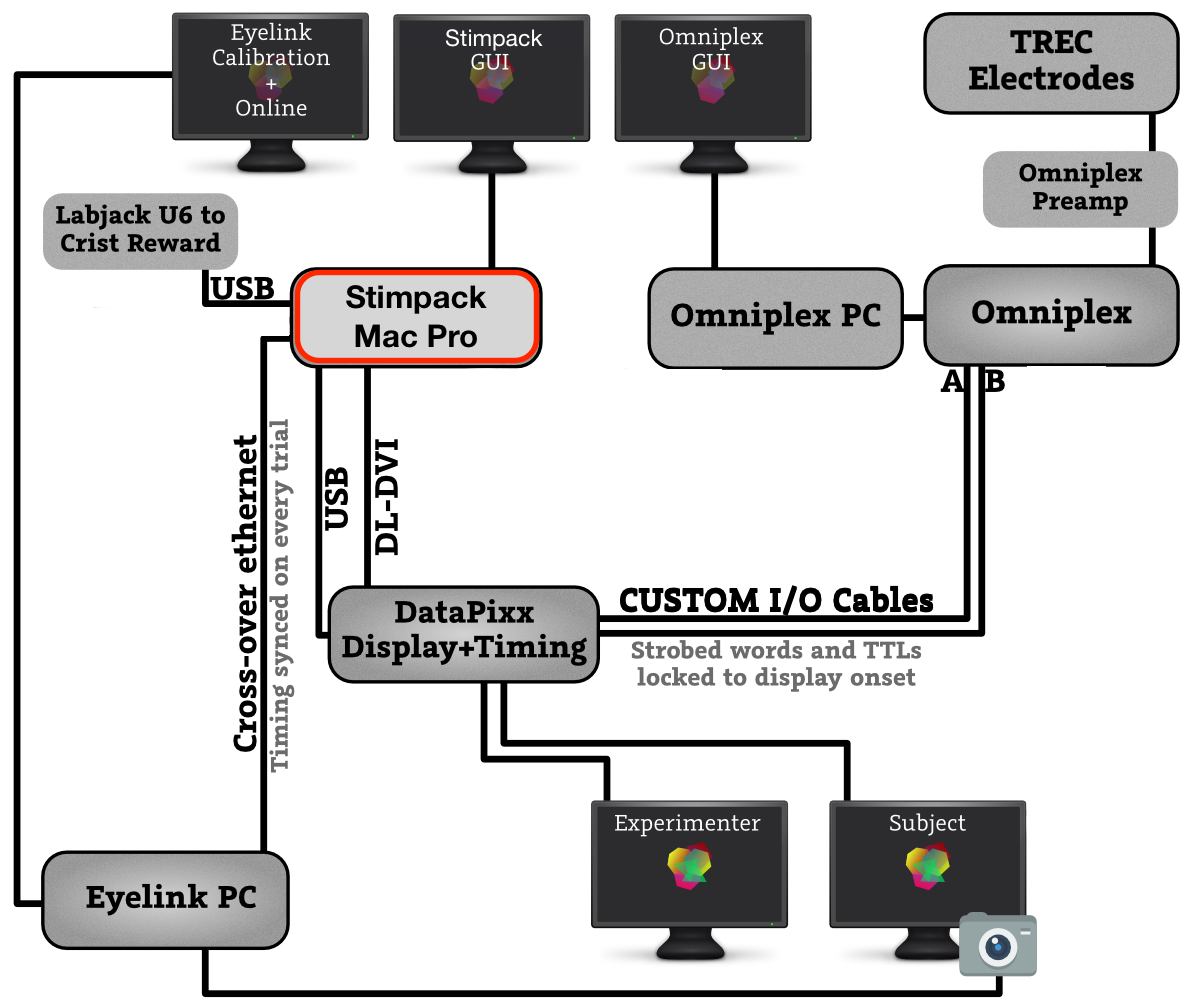
\includegraphics[width=\linewidth]{figures/system_diagram.png}}
\caption{Diagrama de conexiones del sistema.}
\label{figSysDiagram}
\end{figure}
En la figura \ref{figSysDiagram} se puede ver un esquema de las conexiones del sistema. La herramienta se ejecuta en un Mac Pro siendo además necesarios dos equipos adicionales, uno ejecutando Windows empleado para la captura de datos y marcas temporales y otro que forma parte del sistema de seguimiento ocular.

Para el seguimiento ocular se emplea un sistema Eyelink 1000 Plus\cite{eyelink} capaz de realizar un seguimiento binocular a una tasa de muestreo de 2000Hz conectado con el equipo ejecutando Stimpack a través de ethernet.

Para la presentación de estímulos visuales y el envío de marcas temporales se emplea un DATAPixx \cite{datapixx} de VPixx Technologies, conectado al equipo ejecutando la herramienta mediante USB para el envío de marcas temporales y mediante DVI para la presentación de estímulos, esta señal es duplicada en dos monitores, uno que se muestra al sujeto experimental y uno para que el usuario supervise la ejecución del experimento.

Para la captura de datos de los electrodos y de las marcas temporales se emplea un OmniPlex Neural Data Acquisition System\cite{omniplex} de Plexon, conectado al DATAPixx y al preamplificador de los electrodos, también de Plexon. El procesado de estos datos se lleva a cabo en el equipo Windows mencionado anteriormente.

Para la administración de recompensas al animal se emplea un sistema de recompensa digital Crist Instruments V2 Models D1 manejado a través de una  tarjeta de IO digital Labjack U6\cite{labjack}, que se conecta a través de USB con el ordenador que ejecuta la herramienta.


\subsection{Software necesario}
El equipo en el que se utiliza la herramienta funciona sobre OSX 10.9 Mavericks. Tiene instalada una copia de Matlab versión 2015b, la Psychophysics Toolbox v3, la toolbox de Eyelink, la toolbox de Datapixx y la librería para utilizar el Labjack.
El equipo conectado al Omniplex tiene instalado el software Plexcontrol\cite{plexcontrol} para la captura de datos y funciona sobre Windows 7.
El equipo que controla el Eyelink es proporcionado por la empresa fabricante del equipo y se desconoce el software instalado.

\section{Desarrollo}


En esta sección se aborda el desarrollo de Stimpack. 
Según se explico en la introducción, la necesidad de su desarrollo se justifica por la necesidad de una herramienta que se adecue a las necesidades de Neurocom, ya que las herramientas disponibles actualmente son demasiado complejas o bien no compatibles con el hardware del laboratorio.
A lo largo de este apartado se explica tanto el diseño conceptual de la herramienta, como la arquitectura del software y el diseño de la interfaz gráfica de usuario, lo que permite ilustrar como Stimpack satisface los requerimientos deseados para el sistema.  


\subsection{Concepto}
 
 A nivel conceptual Stimpack busca ser una alternativa más ágil de usar que las herramientas existentes en el estado del arte, sacrificando la versatilidad de estas para conseguir una experiencia de usuario más satisfactoria.
 
 La interfaz de usuario debe ser fácil de utilizar y lo más autoexplicativa posible, además debe poder controlar la ejecución del experimento en tiempo real tanto permitiendo pausar o parar la tarea en curso como permitiendo cambiar sus parámetros una vez comenzada.
 
 Para conseguir una interfaz con estas características Stimpack define una ventana separada para cada tarea en vez de usar una interfaz de configuración general para todas las tareas. Estas interfaces siguen una estructura similar, lo que permite que una vez el usuario sepa trabajar con una de las tareas pasar a utilizar otra diferente, solo variando en las partes específicas para cada tarea.
 
 El control del experimento y la supervisión del mismo se llevan a cabo a través de esta misma interfaz, evitando así tener que usar el teclado para enviar comandos, aunque esta opción también está disponible, todo el control, pausar, reanudar, administrar recompensas, etc., se puede realizar con el ratón en la propia interfaz, mientras que cambiando los propios campos de configuración de la tarea, estos parámetros cambiarán en la siguiente iteración del experimento. 

Otra característica deseada para la herramienta es que  sea extensible. Esto se consigue mediante un sistema de plantillas para las tareas, abstrayendo al programador de las nuevas de programar partes no relevantes para la tarea y dejándole centrarse únicamente en las partes importantes de la misma.

%Partiendo de los requisitos expuestos en la sección de objetivos, se decidió desarrollar una herramienta que primara la sencillez ante la capacidad de realizar muchas tareas diferentes por ello se evitó el uso de una única pantalla de configuración, como las usadas en Opticka o Monkeylogic, a favor de interfaces individuales para cada tarea. 

%Estas interfaces siguen una estructura similar, compartiendo la parte donde se especifican las variables experimentales comunes a todas las tareas, como podría ser el color del fondo, tiempo entre ensayos, tamaño del punto de fijación, y completándola con las diferentes variables o formas de control específicas a cada tarea diferente. En esta interfaz se integra además el sistema de control experimental que permite, una vez iniciado el experimento, controlar la ejecución del mismo, ya sea visualizando datos relevantes a cada tarea, mediante una zona de visualización de gráficos, como pausando o deteniendo el experimento, enviando marcas al sistema de registro o administrando manualmente una recompensa al sujeto, todo ello a través de la interfaz gráfica, sin la necesidad de ejecutar comandos de consola ni memorizar combinaciones de teclas. 

%Otra característica de la herramienta es la capacidad de modificar los parámetros del experimento sin necesidad de reiniciarlo, siendo posible cambiar cualquiera de las variables experimentales a través de la interfaz de usuario a tiempo real viendo reflejados los cambios al inicio del siguiente ensayo.
%Ya que se quería que la herramienta fuera expansible, dadas las limitaciones de Matlab a la hora de crear interfaces, se decidió crear una plantilla de tarea, que el desarrollador puede completar para implementar nuevos experimentos.



\subsection{Arquitectura}

\begin{figure*}[htbp]
\centerline{\includegraphics[width=\linewidth]{figures/concept_diagram.png}}
\caption{Diagrama de arquitectura de la herramienta.}
\label{figConceptDiagram}
\end{figure*}



\begin{figure}[bp]
\centerline{\includegraphics[scale=0.15]{figures/class_diagram.png}}
\caption{Estructura de clases que representa a las tareas.}
\label{figClassDiagram}
\end{figure}

Stimpack está estructurado siguiendo una arquitectura por capas, como se puede ver en la figura \ref{figConceptDiagram}. 
\begin{itemize}
	\item La capa UI, donde se definen las múltiples interfaces de usuario.
	\item La capa Task, donde se define la lógica de las diferentes tareas experimentales.
	\item La capa Device Access, que abstrae a las tareas de la complejidad de la interacción con el hardware.
	\item La capa Configuration, transversal al resto de capas responsable de gestionar la configuración básica del sistema.
\end{itemize}
La herramienta cuenta con una clase que hace el papel de lanzador de la aplicación, que es la que se llama al ejecutar la misma. Esta clase crea una instancia de la clase de propiedades, en la que se definen los parámetros básicos de la aplicación. En la implementación actual de la herramienta estas propiedades se pueden diferenciar en tres grupos diferentes: 

\begin{itemize}
	\item Estado de activación del hardware.
	\item Parámetros de ejecución de Psychtoolbox.
	\item Dimensiones del monitor de estimulación.
\end{itemize}

Estas propiedades se pueden modificar desde la ventana principal de la aplicación, que es arrancada por el lanzador del sistema. Desde esta interfaz también se pueden arrancar las IU especificas de cada tarea, que a su vez, instancian y configuran a las clases que implementan la lógica de las tareas.

Estas tareas (figura \ref{figClassDiagram}) son creadas extendiendo una clase abstracta, \textit{AbstractTask}, en la que se definen los parámetros que son comunes a todas las tareas, como pueden ser:

\begin{itemize}

	\item Resolución de la pantalla.
	\item Parámetros de la parte de fijación.
	\item Número de ensayos por tarea.
	\item Tiempo entre ensayos y la variabilidad del mismo.
	\item El estado del experimento.

\end{itemize}

%La clase abstracta cuenta con un método plantilla, \textit{runStimulus}, que se encarga de llamar en orden correcto a los métodos necesarios para la ejecución de la tarea, en una especie de patrón estrategia. Dos de estos métodos, \textit{runTrials} y \textit{endExperiment}, son abstractos y deben ser implementados por las diferentes tareas, definiendo una lógica especifica para cada una.
La clase abstracta cuenta con un método, \textit{RunStimulus} que se encarga de llamar en orden correcto a los métodos necesarios para la ejecución de la tarea.
Dicho método se ha diseñado de acuerdo con el patrón Método Plantilla, de modo que los pasos que  son específicos de una tarea concreta se difieren a la subclase correspondiente.
Asimismo también existen propiedades abstractas, como el nombre de la tarea, que deben ser definidas por cada implementación diferente.
El resto de métodos son los mismos para todas las tareas y se encargan de la preparación del entorno para la ejecución de la tarea, desde la conexión y configuración de los distintos elementos de hardware, configurar la pantalla en la que se mostrarán los estímulos o realizar la limpieza posterior a la ejecución de la tarea.

Además de estos métodos, la clase proporciona algunas funciones que son de utilidad a la hora de programar las tareas, estos métodos de utilidad permiten:

\begin{itemize}
	\item Obtener las coordenadas visuales.
	\item Forzar la actualización de los datos en el visor de la cámara.
	\item Dibujar el punto de fijación.
	\item Comprobar si hay errores en la cámara.
	\item Comprobar los comandos enviados desde la interfaz de control.
\end{itemize}

Esta clase delega en la capa \textit{Device Access} para el acceso a los diferentes dispositivos hardware, empleando las distintas librerías proporcionadas por los fabricantes de los mismos.


%Stimpack está desarrollado usando orientación a objetos para poder implementar un sistema lo más modular posible y facilitar la expansión de la herramienta añadiendo nuevas características.
%Stimpack está formado por varias clases, la clase principal del programa \textit{stimpack} contiene una referencia a la clase de propiedades generales del sistema, de la que se hablará a continuación, y se encarga del inicio de la interfaz gráfica de usuario. Esta clase hereda de la clase \textit{handle} de Matlab, lo que permite su acceso como referencia. La interfaz gráfica principal, arrancada al ejecutar la herramienta, contiene tres botones para arrancar las diferentes tareas y una zona con opciones de configuración.
%La clase \textit(stimprops), que también hereda de handle, contiene las propiedades generales del sistema, como el tamaño real de la pantalla en centímetros y la distancia a la misma, el estado de activación del hardware, el índice del monitor de estimulación, etc, que no necesitan ser cambiadas durante las distintas ejecuciones del experimento.
%Para evitar la repetición de código y abstraer a los futuros desarrolladores de la herramienta de tener que repetir la configuración del sistema en cada tarea diferente se definió una clase abstracta \textit{abstractStimulus} donde se aglomeran todas las propiedades y métodos comunes a todas las tareas, dejando que el  programador de la tarea se centre en la parte más especifica de las tareas, la presentación de estímulos y el procesado de los resultados.

%Algunas de las propiedades mas relevantes definidas en esta clase abstracta son las siguientes:

%\begin{itemize}

%	\item Resolución de la pantalla
%	\item Parámetros de la parte de fijación
%	\item Número de ensayos por tarea
%	\item Tiempo entre ensayos y la variabilidad del mismo
%	\item El estado del experimento

%\end{itemize}

%Además de esas propiedades, existen algunas propiedades abstractas que deben ser implementadas por las tareas que hereden de la clase, que configuran los nombres y las rutas que se emplearan a la hora de guardar los datos al finalizar el experimento.

%Además de las propiedades, en esta clase están definidos los métodos de configuración comunes a todos las tareas, como la configuración de los distintos elementos de hardware que integran el sistema (Eyelink, dataPixx y labJack), la conexión a los mismos, la preparación de la pantalla y la configuración de psychToolbox para la presentación de estímulos y los métodos de limpieza que se ejecutan al terminar el experimento. También está aquí definido el método principal de ejecución de la tarea, que ejecuta todos los métodos en el orden correcto, incluyendo los dos métodos abstractos que el programador debe implementar. Estos métodos son \textit{runTrials} donde se implementa toda la lógica del experimento y \textit{endExperiment} que se ejecuta inmediatamente después de terminar todos los ensayos y cuya finalidad es procesar los datos recogidos en el experimento.

%Aparte de los métodos mencionados anteriormente, \textit{abstractStimulus} proporciona una serie de métodos de utilidad que facilitan la implementación de las tareas:

%\begin{itemize}
%	\item Obtener las coordenadas visuales
%	\item Escribir los datos del ensayo al archivo EDF
%	\item Dibujar el punto de fijación
%	\item Comprobar si hay errores en la cámara
%	\item Comprobar los comandos enviados desde la interfaz de control
%\end{itemize}

\subsection{Interfaz gráfica de usuario}
\begin{figure}[tp]
\centerline{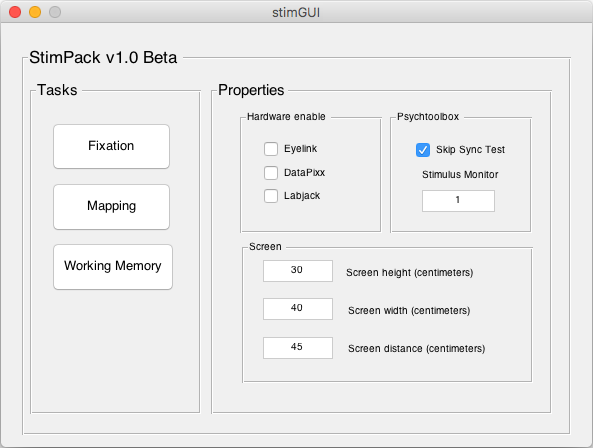
\includegraphics[width=\linewidth]{figures/main_gui}}
\caption{Interfaz principal de la aplicación.}
\label{figmainGUI}
\end{figure}
Como se introdujo en el primer punto, uno de los objetivos de este proyecto es que la herramienta cuente con una interfaz de usuario amigable, que facilite la configuración y control de los experimentos por cualquier investigador sin necesidad de una formación tecnológica especifica.
La interfaz de usuario principal (figura \ref{figmainGUI}) del programa permite el lanzamiento de las diferentes tareas y cuenta con una parte de configuración donde se pueden modificar los siguientes parámetros generales de la aplicación:
\begin{itemize}
	\item La distancia al monitor.
	\item Las dimensiones del monitor.
	\item Activación del sistema de seguimiento ocular.
	\item Activación del sistema de envío de marcas temporales.
	\item Activación del sistema de recompensa.
	\item Activación del modo inseguro de Pychtoolbox.
	\item Selección del monitor de estimulación.
\end{itemize} 

\begin{figure}[tp]
\centerline{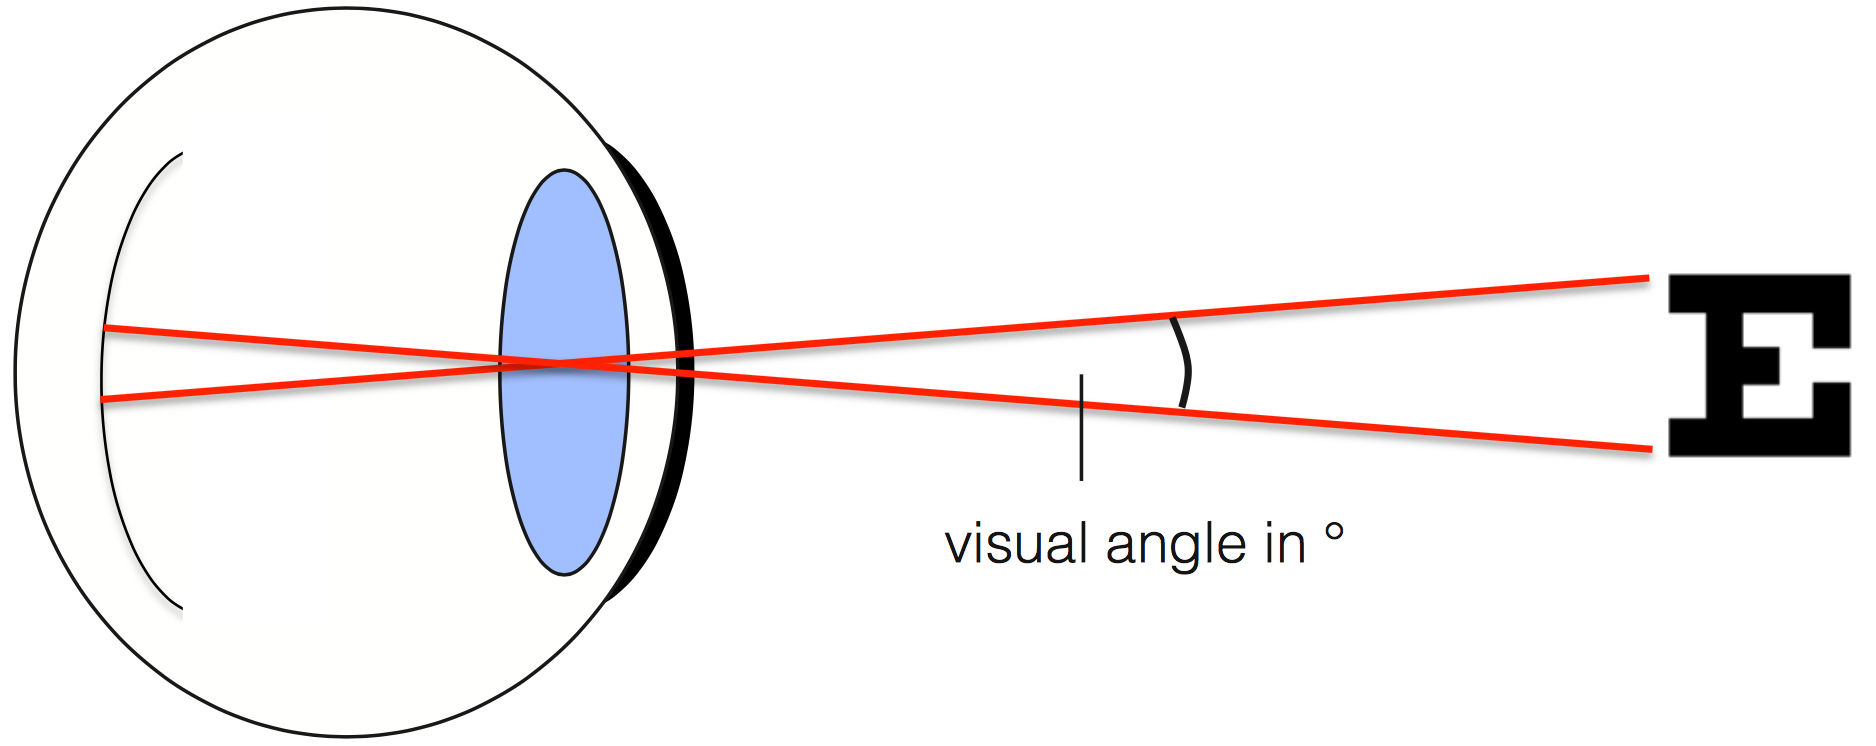
\includegraphics[width=\linewidth]{figures/visual_degrees}}
\caption{Grados del sistema visual.}
\label{figvisualDegrees}
\end{figure}

Las dimensiones y la distancia al monitor son necesarias para calcular la correspondencia en grados del sistema visual y píxeles en la pantalla. Los grados del sistema visual son la unidad tamaño usada en los experimentos que implican visión y permiten trasladar tamaños reales a su proyección en la retina (figura \ref{figvisualDegrees}).

El resto de las opciones son útiles a la hora de desarrollar nuevas tareas o modificar la herramienta, ya que permiten ejecutarla sin la necesidad de contar con todo el equipo. En el caso del sistema de seguimiento visual, si se encuentra desactivado, se puede usar el ratón del ordenador para emular la mirada, en los otros casos, tener el hardware desactivado provoca que se generen logs en la consola para poder depurar la aplicación.

El modo no seguro de Psychtoolbox nos permite ejecutar la aplicación saltándose los tests automáticos de sincronía del monitor. Esta opción es útil cuando es necesario hacer pruebas en monitores que no alcanzan la precisión mínima requerida de sincronía, pero debe ser evitada a la hora de ejecutar experimentos reales ya que los resultados pueden perder precisión.

Las interfaces de las distintas tareas (figuras \ref{figfixGUI}, \ref{figmappingGUI}, \ref{figMemoryGui}) siguen todas una misma estructura, con una parte a la derecha donde se pueden configurar los parámetros de la tarea mediante campos de texto o controles más específicos para cada tarea, y una zona a la izquierda que permite controlar el estado del experimento, con una zona que permite mostrar gráficos del experimento en curso y una serie de botones para controlar la ejecución.

Existe una plantilla básica derivada de la interfaz de la tarea de fijación (figura \ref{figfixGUI}) que se debe usar a la hora de implementar nuevas tareas.
Los detalles de las interfaces especificas de cada tarea son tratadas con mayor detalle en el siguiente apartado.

\subsection{Tareas implementadas}

Para el desarrollo del experimento explicado en el primer apartado, ha sido necesario implementar tres tareas diferentes en Stimpack:
\begin{itemize}
	\item La tarea de fijación, usada para entrenar al mono a fijar la mirada en un punto.
	\item La tarea de mapeo, que permite buscar los campos receptores en la corteza visual. 
	\item La tarea de memoria de trabajo, que permitirá comprobar la hipótesis planteada por el proyecto.
\end{itemize}
Estas tres tareas fueron incluidas en esta implementación de la herramienta. Adicionalmente se creó una plantilla a partir de la primera (fijación) para desarrollar nuevas tareas sin tener que reescribir el código común. 
A continuación se extienden los detalles de cada tarea individualmente.

\subsubsection*{Tarea de fijación}
\begin{figure*}[tp]
\centerline{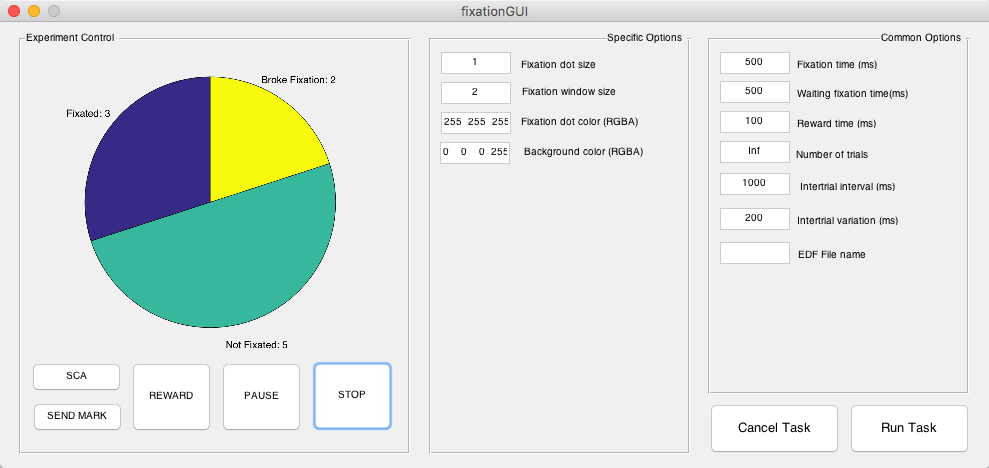
\includegraphics[width=\linewidth]{figures/fixation_gui}}
\caption{Interfaz de la tarea de fijación.}
\label{figfixGUI}
\end{figure*}

\begin{figure}[bp]
\centerline{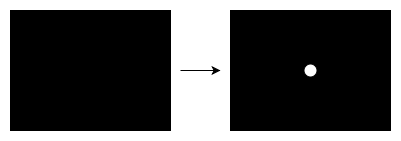
\includegraphics[width=\linewidth]{figures/fixation}}
\caption{Tarea de fijación.}
\label{figfixTask}
\end{figure}



La tarea de fijación es la más básica de las implementadas y sirve de base para el resto, derivando la plantilla para crear tareas directamente de esta. 
En la tarea de fijación se le muestra al individuo un punto sobre un fondo en el que debe fijar la vista. Si lo hace correctamente se le da una recompensa.
Los pasos de la tarea son los siguientes:

\begin{enumerate}
	\item Aparece solo el fondo.
	\item Aparece el punto de fijación.
	\item El sujeto tiene un tiempo limite para poner la mirada sobre el punto.
	\item Una vez tiene la mirada fija en el punto, debe permanecer un tiempo definido.
	\item Desaparece el punto y si ha hecho correctamente todos los pasos se le da una recompensa.
	\item Tiempo entre ensayos y vuelta al punto 1.
\end{enumerate}

En la figura \ref{figfixTask} puede verse lo que se le muestra al sujeto durante el experimento. 

Esta tarea sirve para entrenar al sujeto en mantener la mirada en el punto de fijación. Es necesario entrenar al sujeto en mantener la vista fija en el punto de fijación, ya que en el resto de tareas es un requisito indispensable que el animal mantenga la mirada en todo momento en el punto de fijación.

Esta tarea es totalmente parametrizable, de forma muy sencilla, pudiéndose modificar a través de la interfaz gráfica (figura \ref{figfixGUI}) las siguientes propiedades:
\begin{itemize}
	\item Tamaño del punto de fijación y de la ventana de fijación.
	\item Color del punto de fijación y del fondo.
	\item Tiempo de espera de fijación.
	\item Tiempo de fijación.
	\item Tiempo de recompensa.
	\item Tiempo entre ensayos.
	\item Variación del tiempo entre ensayos.
	\item Número de ensayos.
\end{itemize}

Durante el experimento, se le muestra al investigador en la interfaz de usuario un gráfico de sectores donde se puede ver la cantidad de ensayos terminados con éxito, abortados por romper la fijación o fallidos por no haber alcanzado la fijación, esto ayuda a saber que tal progresa el experimento, pudiendo decidir si pausar el experimento o pararlo si el animal no progresa en la tarea.

\subsubsection*{Tarea de mapeo}

\begin{figure}[bp]
\centerline{
\includegraphics[width=\linewidth]{figures/mapping_task}}
\caption{Tarea de mapeo.}
\label{figMapTask}
\end{figure}

\begin{figure*}[tp]
\centerline{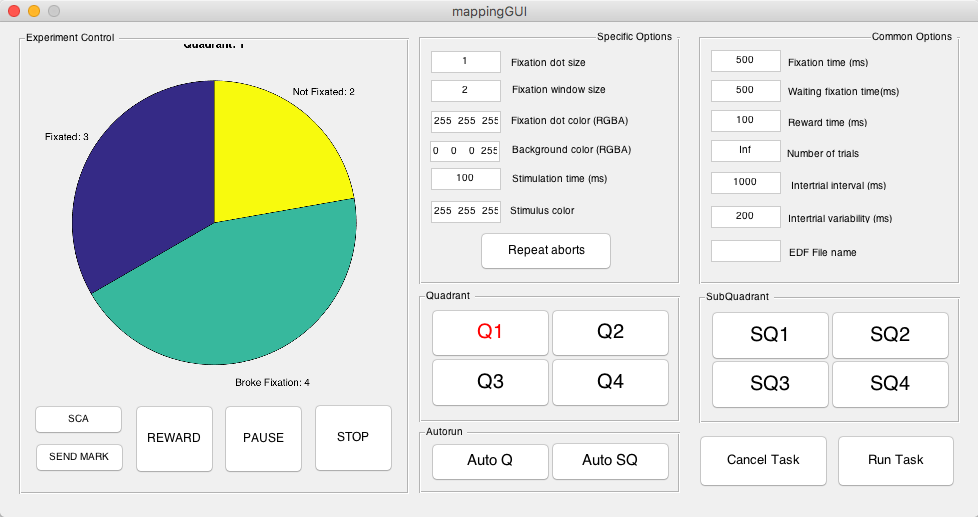
\includegraphics[width=\linewidth]{figures/mapping_gui}}
\caption{Interfaz de la tarea de mapeo.}
\label{figmappingGUI}
\end{figure*}

La tarea de mapeo se construye sobre la tarea de fijación y comparte todos su parámetros, además de añadir parámetros propios y una interfaz gráfica basada en la anterior pero adecuada a esta tarea.
En la tarea de mapeo se le muestra al sujeto el punto de fijación, una vez consigue fijar la mirada aparece un estimulo, en forma de un rectángulo de color. El animal debe seguir manteniendo la mirada en el punto de fijación hasta que desaparezca. Si lo consigue se le da una recompensa.
El protocolo seguido es el siguiente:

\begin{enumerate}
	\item Aparece el fondo.
	\item Aparece el punto de fijación.
	\item El animal fija.
	\item Aparece el estímulo.
	\item El animal mantiene la fijación.
	\item Desaparece el punto y el estímulo.
	\item Recompensa.
	\item Tiempo entre ensayos y vuelta al punto 1.
\end{enumerate}


En la figura \ref{figMapTask} puede verse lo que se le muestra al sujeto durante la tarea. 



Los parámetros modificables adicionalmente a los de la tarea de fijación son el tiempo de presentación del estímulo y el color del mismo. Además cuenta con una serie de botones (figura \ref{figmappingGUI}) que permiten controlar qué estimulo (cuadrante o subcuadrante) se le mostrará al animal, dos botones para activar el ciclado automático de cuadrantes entre ensayos y un botón para en caso de estar activado el ciclado de cuadrantes, repita el último mientras no se realice correctamente.
Los botones están colocados de manera que seleccionar la zona de estimulación sea fácil, rápido e intuitivo, optando por una disposición física de los botones acorde a los estímulos en pantalla en vez de un simple listado de cuadrantes.
Durante el experimento se le muestra al investigador un gráfico similar al de la tarea de fijación, pero mostrando los datos para el cuadrante seleccionado en la interfaz.


Esta tarea permite registrar datos neuronales sobre que neuronas se activan al presentar cierto estímulo en parte de la retina, los denominados campos receptores,  y enfocar con mayor precisión los estímulos futuros.


\subsubsection*{Tarea de memoria de trabajo}

\begin{figure}[bp]
\centerline{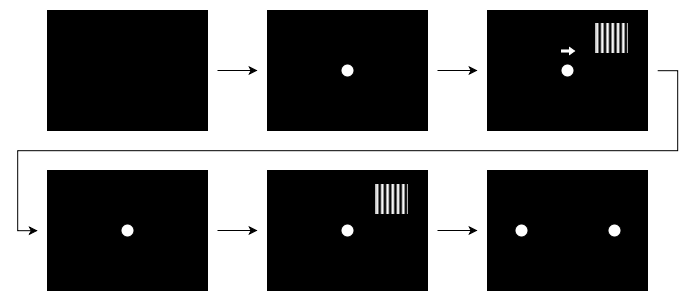
\includegraphics[width=\linewidth]{figures/memory_task}}
\caption{Tarea de memoria de trabajo (con flecha).}
\label{figMemoryTask}
\end{figure}

\begin{figure*}[tp]
  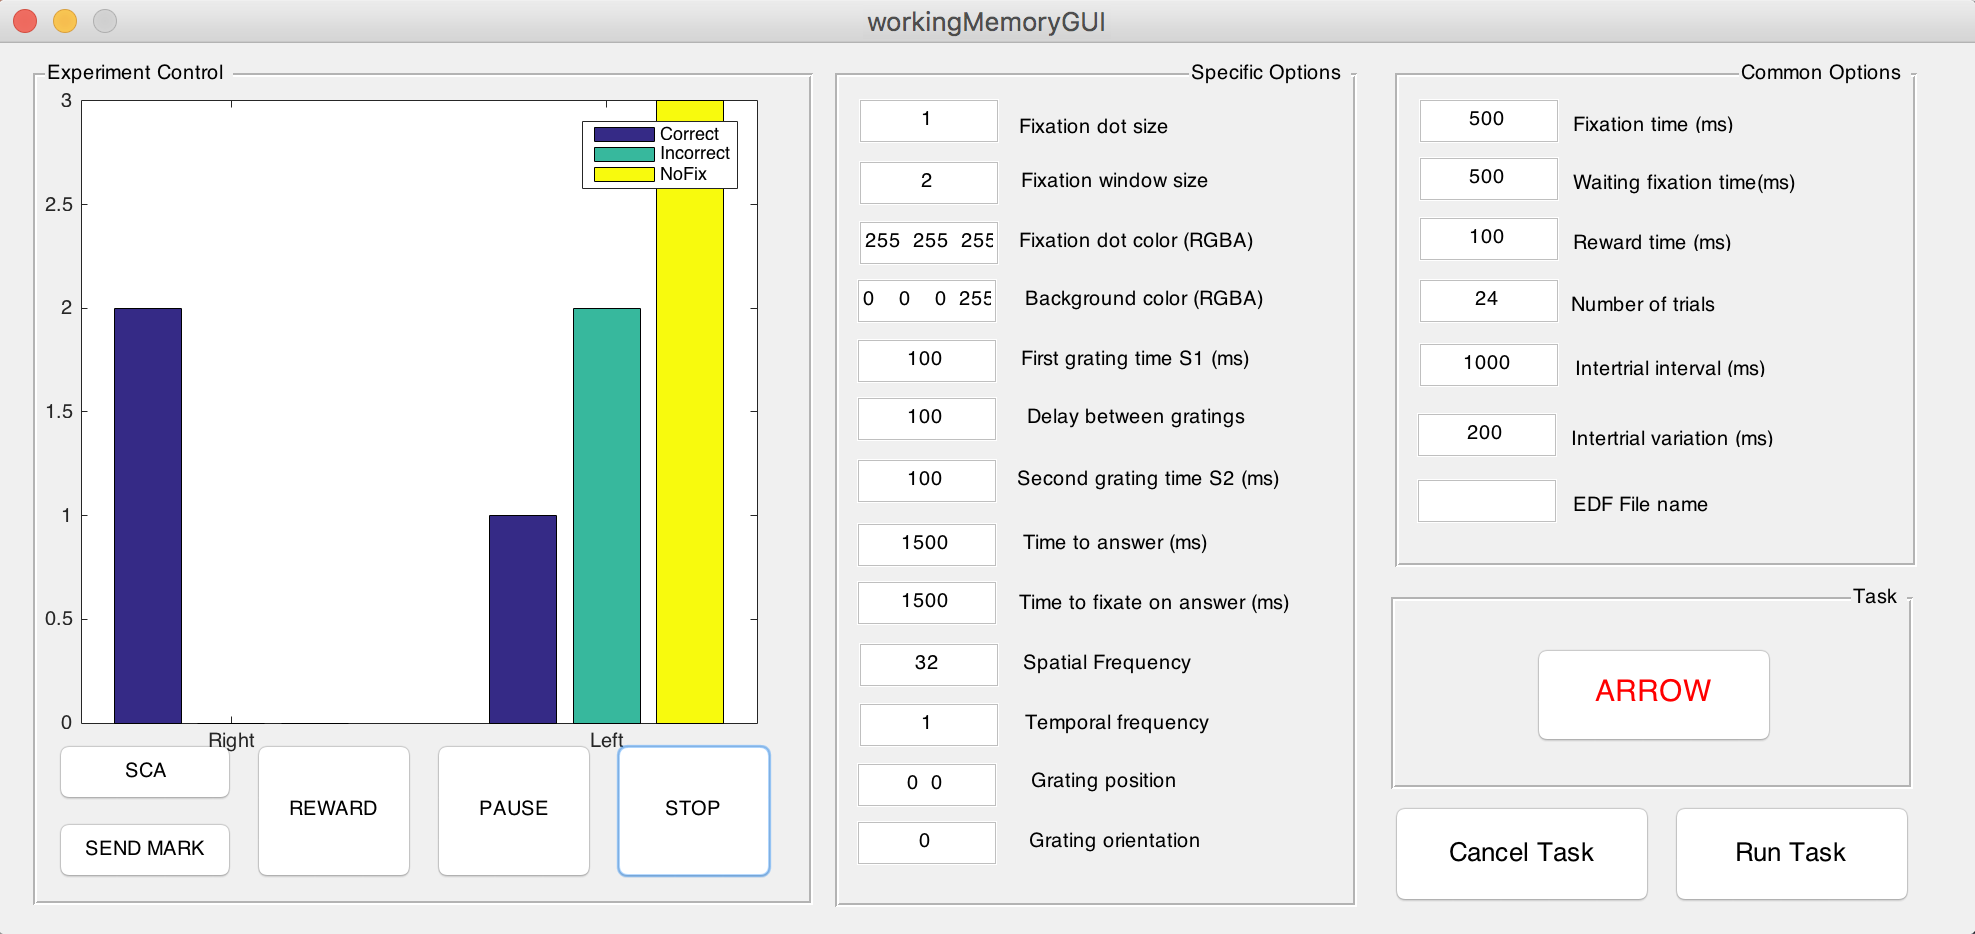
\includegraphics[width=\textwidth]{figures/memory_gui}
  \caption{Interfaz de la tarea de memoria de trabajo}
  \label{figMemoryGui}

\end{figure*}

La última tarea implementada es la más elaborada de todas. Fue construida también sobre la plantilla y es la que se va a utilizar para llevar a cabo la investigación sobre la memoria de trabajo. 
En esta tarea el animal debe fijar la mirada en el punto, una vez fija se le muestra un estímulo, que puede ser de dos tipos diferentes, un grating en movimiento o un grating más una flecha, una vez pasa un tiempo el estimulo desaparece y se deja únicamente el punto de fijación, pasado otro momento se muestra un grating moviéndose en una dirección aleatoria, una vez pasado otro intervalo de tiempo desaparecen tanto el estimulo como el punto de fijación y aparecen dos puntos a los lados de la pantalla. En el caso del estímulo sin flecha, el animal debe fijar la mirada en el punto en el lado hacia el cual se movía el primer grating, en caso de que fuera el con flecha, debe escoger  hacia el lado que señalaba la misma.
Los pasos organizados son los siguientes:


\begin{enumerate}
	\item Aparece punto de fijación.
	\item Animal fija.
	\item Aparece primer estímulo (con o sin flecha).
	\item Desaparece el estimulo y se mantiene el punto de fijación.
	\item Aparece el segundo estímulo (solo grating).
	\item Desaparecen el estímulo y el punto de fijación y aparecen los selectores en el monitor.
	\item El animal escoge fijando la vista en uno de ellos.
	\item Desaparecen los selectores y si escoge el correcto se le da recompensa.
	\item Tiempo entre ensayos y vuelta al punto 1.
\end{enumerate}

En la figura \ref{figMemoryTask} puede verse este proceso. 


Los parámetros modificables son los siguientes:

\begin{itemize}
	\item Tiempo del primer estímulo.
	\item Tiempo entre estímulos.
	\item Tiempo del segundo estímulo.
	\item Tiempo disponible para responder.
	\item Tiempo de fijación en los selectores.
	\item Frecuencia espacial y temporal del grating.
	\item Posición del grating.
	\item Orientación del grating.

\end{itemize}


Además de estos parámetros, en la interfaz gráfica (figura \ref{figMemoryGui}) existe un botón para cambiar entre las dos variantes de la tarea con y sin flecha.
Las direcciones empleadas para el primer estímulo son precalculadas en base al número de ensayos, 50\% hacia cada lado, y después son ordenadas de manera aleatoria.

En la zona de información de la interfaz de usuario se muestra un gráfico de barras separado en izquierda y derecha que muestra las diferentes estadísticas de fijación, no fijación y rotura de fijación para cada lado.


En esta tarea se pone a prueba la memoria de trabajo del sujeto, haciéndole recordar una dirección hasta que aparezcan los selectores. 
En este tiempo se le puede aplicar al sujeto la estimulación magnética transcraneal (TMS) en la corteza prefrontal. Si la hipótesis es correcta, se verá afectado el rendimiento del individuo a la hora de realizar la tarea que implica la flecha ya que requiere información contextual (el animal debe aprender qué significa la flecha), sin embargo la versión sin flecha, al ser una estimulación puramente sensorial, no debería verse afectada.

\section{Conclusiones}

En este trabajo se ha implementado una herramienta que permite el control de experimentos de estimulación visual.

Stimpack proporciona un entorno fácil de utilizar que permite al usuario ejecutar las tres tareas de comportamiento definidas en los objetivos del proyecto, limitando la interacción a través de la línea de comandos únicamente a arrancar propia herramienta. La interfaz gráfica se ha simplificado al máximo, creando ventanas especificas para cada tarea. Esto distancia a la herramienta de otras cómo Opticka o Monkeylogic, que cuentan con interfaces de usuario muy densas y genéricas. Esta característica de stimpack lo hace más usable a costa de una menor flexibilidad.

Stimpack emplea como lenguaje de programación Matlab y como framework para la presentación de estímulos Psychtoolbox, herramientas que se han convertido en el estándar para el desarrollo de experimentos de psicofísica y neurociencia.

Se proporciona una forma de expandir la herramienta con nuevas tareas haciendo uso de plantillas, donde los desarrolladores solo necesitan centrarse en la programación de la tarea y la presentación de estímulos, despreocupándose de la parte de configuración y conexión a los diferentes sistemas de hardware.

La herramienta se integra con los sistemas de seguimiento ocular y adquisición de datos disponibles en el laboratorio, permitiendo una transición suave desde la herramienta anterior, sin necesidad de cambiar ningún elemento del sistema.

Durante el desarollo se ha mantenido una comunicación con los investigadores al cargo del proyecto y se han realizado pruebas en el entorno real, lo que ha permitido que la herramienta se adapte bien a sus necesidades. Stimpack comenzará a emplearse en breve en el proyecto sustituyendo a Opticka en el desarrollo de los experimentos.

La herramienta está publicada en un repositorio público en Github\cite{stimpackrepo} y se espera que a través del feedback proporcionado los usuarios pueda convertirse en una herramienta general para estimulación visual y no sólo algo especifico para este experimento.

\section{Agradecimientos}

Quiero agradecer a Juan Casto Rivadulla Fernández por la dirección de este proyecto, a Sandra Yaneth Prieto Soler y José Luis Pardo Vázquez por su ayuda en el laboratorio y sus consejos desde la perspectiva de investigadores para desarrollar la herramienta. 
También quiero agradecer la ayuda prestada por Alejandro Paz López cuyos consejos, permitieron la mejora de la arquitectura del sistema.

\begin{thebibliography}{00}
\bibitem{neurocom1} Aguila, J., Cudeiro, F. J. and Rivadulla, C. (2017) ‘Suppression of V1 Feedback Produces a Shift in the Topographic Representation of Receptive Fields of LGN Cells by Unmasking Latent Retinal Drives’, Cerebral Cortex, 27(6), pp. 3331–3345. doi: 10.1093/cercor/bhx071.

\bibitem{neurocom2} Ortuño, T. et al. (2014) ‘Bursting thalamic responses in awake monkey contribute to visual detection and are modulated by corticofugal feedback’, Frontiers in Behavioral Neuroscience, 8(May), pp. 1–10. doi: 10.3389/fnbeh.2014.00198.

\bibitem{cortex} Cortex: A Program for COmputerized Real Time EXperiments. http://www.cnbc.cmu.edu/~rickr/ctxman5.html (Online) Último acceso: 14/6/2018


\bibitem{monkeylogic}ASAAD, Wael F.; ESKANDAR, Emad N. A flexible software tool for temporally-precise behavioral control in Matlab. Journal of neuroscience methods, 2008, vol. 174, no 2, p. 245-258.


\bibitem{psychtoolbox} BRAINARD, David H.; VISION, Spatial. The psychophysics toolbox. Spatial vision, 1997, vol. 10, p. 433-436.

\bibitem{psychopy} Peirce, J. W. (2007) ‘PsychoPy—Psychophysics software in Python’, Journal of Neuroscience Methods. Elsevier, 162(1–2), pp. 8–13. doi: 10.1016/J.JNEUMETH.2006.11.017.

\bibitem{wave} Meyer, T. and Constantinidis, C. (2005) ‘A software solution for the control of visual behavioral experimentation’, Journal of Neuroscience Methods, 142(1), pp. 27–34. doi: 10.1016/j.jneumeth.2004.07.009.

\bibitem{opticka} Opticka visual stimulus generator. http://iandol.github.io/opticka/ (Online) Último acceso: 16/6/2018


\bibitem{omniplex} OmniPlex Neural Data Acquisition System. https://plexon.com/products/omniplex-d-neural-data-acquisition-system-1/ (Online) Último acceso: 13/6/2018

\bibitem{eyelink} Eyelink 1000 Plus Eye Tracking System. https://www.sr-research.com/products/eyelink-1000-plus/ (Online) Último acceso: 13/6/2018
\bibitem{datapixx} VPixx Technologies DATAPixx data acquisition and graphics toolbox. http://vpixx.com/products/tools-for-vision-sciences/display-drivers/datapixx/  (Online) Último acceso: 13/6/2018

\bibitem{plexcontrol} Plexcontrol Software. https://plexon.com/products/omniplex-software/ (Online) Último acceso: 18/6/2018

\bibitem{labjack} Labjack U6 DAQ. https://labjack.com/products/u6 (Online) Último acceso: 13/6/2018




\bibitem{stimpackrepo} Stimpack repository. https://github.com/Shiul93/stimpack (Online) Último acceso: 18/6/2018

\end{thebibliography}

\vspace{12pt}


\end{document}
